\section{Introduction to Compartmental Models}

\begin{frame}{Why Model Epidemics?}
  \begin{itemize}
    \item Infectious diseases have shaped human history: plague, smallpox, influenza, COVID-19.
    \vfill
    \pause
    \item \textbf{Mathematical models} allow us to:
      \begin{itemize}
        \item Understand \textbf{how} and \textbf{why} epidemics spread.
        \item Predict the course of an outbreak \textbf{before} it unfolds.
        \item Evaluate \textbf{interventions} (vaccination, quarantine, social distancing).
        \item Estimate key quantities: peak hospital load, total infections, epidemic duration.
      \end{itemize}
    \pause
      \vfill
    \item Models are \textbf{simplifications} of reality --- but useful ones.
    \item \textit{``All models are wrong, but some are useful.''} --- George E.\ P.\ Box
  \end{itemize}
\end{frame}

\begin{frame}{Compartmental Models: The Core Idea}
  \begin{itemize}
    \item Divide the population into \textbf{compartments} based on disease status.
    \item Individuals move between compartments according to \textbf{transition rules}.
    \item Each transition has a \textbf{rate} that depends on the current state of the population.
  \end{itemize}
  \vfill
  \begin{center}
    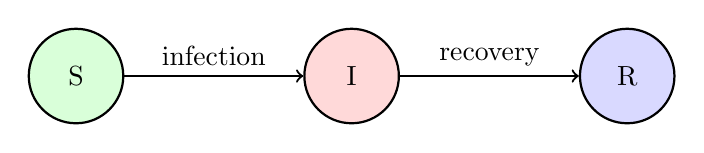
\begin{tikzpicture}[node distance=3.5cm]
      \node[draw, circle, thick, minimum size=1.2cm, fill=green!15] (S) {S};
      \node[draw, circle, thick, right of=S, minimum size=1.2cm, fill=red!15] (I) {I};
      \node[draw, circle, thick, right of=I, minimum size=1.2cm, fill=blue!15] (R) {R};
      \draw[->, thick] (S) -- node[midway, above] {infection} (I);
      \draw[->, thick] (I) -- node[midway, above] {recovery} (R);
    \end{tikzpicture}
  \end{center}
  \vfill
  \small
  Example: the SIR model. Susceptible $\to$ Infected $\to$ Recovered.
\end{frame}

\begin{frame}{Two Approaches to Epidemic Modeling}
  \begin{columns}[t]
    \column{0.48\textwidth}
    \textbf{Equation-based (ODE) models}
    \begin{itemize}
      \item Track \textbf{population fractions} ($S$, $I$, $R$).
      \item Described by differential equations.
      \item Deterministic --- same parameters always give the same result.
      \item Assume a \textbf{well-mixed} population.
      \item Fast to compute, easy to analyse mathematically.
    \end{itemize}
  \pause
    \column{0.48\textwidth}
    \textbf{Agent-based models (ABM)}
    \begin{itemize}
      \item Track \textbf{individual agents} with their own state and position.
      \item Rules applied to each agent separately.
      \item Stochastic --- different runs give different outcomes.
      \item Can include \textbf{space}, \textbf{networks}, \textbf{heterogeneity}.
      \item More realistic, but harder to analyse.
    \end{itemize}
  \end{columns}
  \vfill
\end{frame}

\begin{frame}{Key Concepts We Will Cover}
  \begin{enumerate}
    \item \textbf{Compartmental ODE models}: SI, SIS, SIR, SEIR
      \begin{itemize}
        \item Differential equations, equilibria, stability analysis
        \item Basic reproduction number $R_0$ and herd immunity
      \end{itemize}
    \vfill \pause
    \item \textbf{Agent-based SIR model}
      \begin{itemize}
        \item Individual agents, random movement, contact-based infection
        \item Stochastic variability and spatial effects
      \end{itemize}
    \vfill \pause
    \item \textbf{Comparative analysis}
      \begin{itemize}
        \item When do ODE and ABM agree? When do they differ?
        \item Effect of population size, vaccination strategies
      \end{itemize}
  \end{enumerate}
\end{frame}

\begin{frame}{A Brief History of Epidemic Modeling}
  \footnotesize
  \begin{itemize}
    \item \textbf{1760} --- Daniel Bernoulli: first mathematical analysis of smallpox inoculation.
    \item \textbf{1906} --- W.\ H.\ Hamer: discrete-time model of measles --- introduced the \textbf{mass action principle} (infection rate $\propto S \times I$).
    \item \textbf{1927} --- Kermack \& McKendrick: the classical \textbf{SIR model} and the epidemic threshold theorem.
    \item \textbf{1950s--70s} --- Extensions: SIS, SEIR, age-structured models, vital dynamics.
    \item \textbf{1990s--2000s} --- Agent-based and network models become computationally feasible.
    \item \textbf{2020} --- COVID-19 pandemic: models (ODE, ABM, network) used worldwide for policy decisions, forecasting, and vaccination planning.
  \end{itemize}
  \vfill
  \pause
    \footnotesize
  \begin{block}{The mass action principle}
    The rate of new infections is proportional to the product of susceptible and infected individuals: $\beta S I$. This is the foundation of all compartmental models.
  \end{block}
\end{frame}




